\subsection{系统性能测试}
\label{sub:evaluation-performance}


\paragraph{Setup.} 我们为性能评估配置了两个测试平台。

\begin{itemize}[leftmargin=*]
\item {\bf LAN.} 它包括三台机器,每台机器配备一个八核 2.9\,GHz Intel Core i7-10700 CPU,一个 4\,TB 7200 RPM Seagate Exos SATA 硬盘驱动器和 32\ ,GB 内存。所有机器都通过 10\,Gbps 交换机连接,并运行 Ubuntu 20.04.3。

\item {\bf Cloud.} 部署在 {\em 阿里云} \cite{alibaba}。我们在两个区域租用了几台 {\em ecs.g7t.3xlarge} 虚拟机 (VM) 来分别运行云、关键服务器和多个客户端。同一地域和不同地域的虚拟机分别连接 10\,Gbps 和 100\,Mbps 网络。每个 VM 配备一个 12 核 3.5GHz CPU,由 Intel Xeon (Ice Lake) Platinum 8369B 和 48GiB 内存虚拟化,并安装阿里云 Linux 3.2104。我们另外挂载了以 {\em Alibaba General-Purpose NAS} 作为存储后端的云机。 NAS 可实现高达 15K\,IOPS 的 4\,K 次随机读写,带宽为 150\,MBps。
\end{itemize}

我们进行以下默认配置。对于底层\sysnameF,我们固定$W$ = 5\,K(即大约300\,KiB EPC使用量),$T$ = 3\%,相似性指标的大小为32\,bytes(即,两个块),通过 N 变换提取的特征数量为三个。对于 \prototype,我们配置了三个线程来提取明文块的内容特征(除了 Exp\#5,它在单个线程中对 \prototype 的性能进行微基准测试,而 Exp\#6 使用不同的数字来评估 \prototype 的性能用于提取内容特征的线程)和一个 1\,GiB 容器缓存以提高下载性能(\S\ref{sec:implementation})。

\subsubsection{Synthetic Workloads}
\label{subsub:syn}
我们使用 SYNUnique 评估 \prototype,其中每个 2\,GiB 文件包括全局唯一的块 (\S\ref{sub:datasets})。为了避免磁盘 I/O,我们在每次测试之前将所有数据加载到每个客户端的内存中,并让云端将所有接收到的数据存储在内存中(相对于 Exp\#8 使磁盘 I/O 研究真实云部署) .我们的目标是在不影响重复数据删除和磁盘 I/O 的情况下了解 \prototype 可实现的最大性能,并表明 \prototype 与 SGXDedup \cite{ren21} 相比会产生有限的性能开销。我们将每个实验的结果平均超过 10 次,并将 {\em Student's t-Distribution} 的 95\% 置信区间包含在条形图中(为简洁起见,我们将它们从折线图中排除)。

\paragraph{Exp\#5(微基准测试)。}
我们从微基准评估开始,在 LAN 测试平台的不同机器上部署客户端、关键服务器和云。我们让客户端在 SYNUnique 中两次上传相同的 2\,GiB 文件,并在单个线程中评估不同上传步骤的处理时间。考虑的步骤包括: (i) {\em chunking},将输入文件划分为可变大小的明文块; (ii) {\em 特征生成},提取每个明文块的内容特征,并根据 \sysnameF 实例对目标特征进行采样; (iii) {\em 指纹},计算每个明文块的指纹; (iv) {\em key generation},生成特征密钥和 MLE 密钥; (v) {\em encryption},对每个明文块进行加密; (vi) {\em detection},基于密文块检测学习内容攻击; (vii) {PoW},证明每个密文块的所有权; (viii) {\em deduplication},云检测重复块; (ix) {\em transfer},它传输不重复的密文块和文件配方。



\begin{table}[t]
    \small
    \centering
    \setlength{\tabcolsep}{5pt}
    \renewcommand{\arraystretch}{1.05}
    \setlength{\tabcolsep}{0.006\textwidth}{
    \begin{tabular}{|c|c|c|c|c|}
        \hline
        \multicolumn{2}{|@{\,}c|}{\textbf{Procedure/Step}} & \multicolumn{1}{l|}{\hspace{.5em}\textbf{firstFeature}} &
        \multicolumn{1}{c|}{\textbf{minFeature}} &
        \multicolumn{1}{c|}{\textbf{allFeature}} \\ \hline \hline
        \multicolumn{2}{|c|}{Chunking} & \multicolumn{3}{c|}{$2.12\pm0.006$} \\ \hline
        \multicolumn{2}{|c|}{\makecell[c]{Feature generation}} &
        \makecell[c]{$4.34 \pm 0.01$} & \makecell[c]{$9.93 \pm0.04$} & \makecell[c]{$9.85 \pm0.02$} \\ \hline
        \multicolumn{2}{|c|}{\makecell[c]{Fingerprinting}}&
        \multicolumn{3}{c|}{$1.81 \pm 0.002$} \\ \hline        \multicolumn{2}{|c|}{\makecell[c]{Key generation}}&
        \multicolumn{3}{c|}{$0.73 \pm 0.02$ ($0.49 \pm 0.01$)} \\ \hline
        \multicolumn{2}{|c|}{Encryption} & \multicolumn{3}{c|}{$1.22 \pm 0.001$} \\ \hline
        \multirow{2}{*}{In Enclave}
        & Detection &
        \multicolumn{3}{c|}{$0.04   \pm 0.005$} \\ \cline{2-5}
        & PoW &
        \multicolumn{3}{c|}{$1.86   \pm 0.004$} \\ \hline
        \multicolumn{2}{|c|}{Deduplication}  &
        \multicolumn{3}{c|}{$0.55 \pm 0.02$}  \\ \hline
        \multicolumn{2}{|c|}{Transfer}  & \multicolumn{3}{c|}{$1.16 \pm 0.03$ ($0.04 \pm 0.001$)}\\ \hline
    \end{tabular}
    }
    \caption{(Exp\#5) 处理合成文件数据每 1\,MiB 的时间分解(单位:ms)。 除括号中明确指定外,第二次上传的每一步所消耗的时间与第一次上传的相同。}
    \label{tab:evaluation-syn-system-breakdown}
    \vspace{-6pt}
\end{table}
表~\ref{tab:evaluation-syn-system-breakdown} 展示了结果(每 1\,MiB 文件数据处理)。由于 \prototype 建立在 SGXDedup \cite{ren21} 之上,它继承了在第二次上传中卸载密钥生成 (\S\ref{sec:implementation}) 的计算开销以及避免传输重复块的性能优势.检测步骤是高效的,并且在上传过程中占用了总时间的 0.4\%。此外,由于 N 变换的计算开销,特征生成步骤很昂贵。例如,{\tt firstFeature} 在第一次上传时占用了总时间的 31.4\%; {\tt minFeature} 和 {\tt allFeature} 所消耗的时间分数分别进一步增加到 51.1\% 和 50.9\%,因为它们提取了所有三个特征(与只提取第一个特征的 {\tt firstFeature} 相反) )。然而,我们认为我们可以通过多线程来减轻特征生成的性能开销(见下文)。


\paragraph{Exp\#6(单客户端性能)。}
我们考虑单个客户端,并将 \prototype 的性能与基本系统 SGXDedup 进行比较。我们让客户端两次上传相同的文件(如 Exp\#5)并进一步下载文件。


图~\ref{fig:singleClientThroughput}(a) 和Figure~\ref{fig:singleClientThroughput}(b) 分别展示了当我们改变提取特征的线程数(\S\ref{sec:implementation})。 SGXDedup 的速度在第一次上传时保持为 297.1\,MiB/s,在第二次上传时保持为 304.3\,MiB/s,因为它不提取特征。 \prototype 的上传速度首先随着线程数的增加而增加(例如,{\tt firstFeature} 为 265.3\,MiB/s,{\tt minFeature} 为 261.3\,MiB/s,{\tt minFeature} 为 262.6\,MiB/s {\tt allFeature} 当三个线程用于在第一次上传中提取特征时),然后减少(例如,在第一次上传中大约为 220\,MiB/s 和在第二次上传中为 225\,MiB/s 对于所有三个实例)由于资源争用。通过利用多线程,\prototype 仅在第一次上传时比 SGXDedup 产生 8.0-12.0\% 的性能开销,在第二次上传时为 6.6-7.5\%。此外,我们观察到第一次和第二次(不需要传输重复数据)上传之间的性能差异很小,因为我们的 LAN 测试平台具有高带宽来传输数据。我们认为基于数据源的重复数据删除在实际云部署中带来了显着的性能提升(Exp\#8),并减少了处理实际存储工作负载的网络流量(Exp\#10)。图~\ref{fig:singleClientThroughput}(c)比较下载速度。 \prototype 会导致 1.3\% 的性能下降,因为它使用 MLE 密钥和功能密钥解密每个块。


\begin{figure}[t]
    \centering
    
\includegraphics[width=0.7\textwidth]{pic/featurespy/plot/performance/LANSyn/legend.pdf}\\
    \vspace{1pt}
    \begin{tabular}{@{\ }c@{\ }c@{\ }c}
        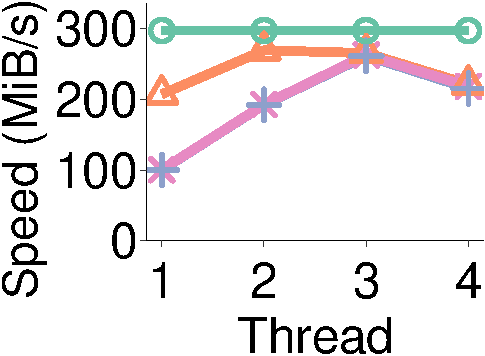
\includegraphics[width=0.32\textwidth]{pic/featurespy/plot/performance/LANSyn/upload_thread_line.pdf}&
        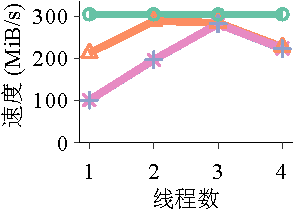
\includegraphics[width=0.32\textwidth]{pic/featurespy/plot/performance/LANSyn/upload_thread_2nd_line.pdf}&
        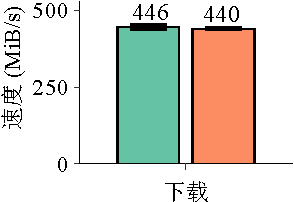
\includegraphics[width=0.32\textwidth]{pic/featurespy/plot/performance/LANSyn/download_bar.pdf}\\
        \makecell[c]{\small (a) 1st upload} &
        \makecell[c]{\small (b) 2nd upload} &
        \makecell[c]{\small (c) Download}\\
    \end{tabular}
    \vspace{-6pt}
    \caption{(Exp\#6) LAN 测试平台中的单客户端性能。 在下载中,所有 \prototype 实例都达到相同的速度,我们将它们(橙色)与 SGXDedup(绿色)进行比较。}
    \vspace{-6pt}
    \label{fig:singleClientThroughput}
\end{figure}

\paragraph{Exp\#7(多客户端性能)。}
我们评估多个客户端同时发出上传/下载时的性能。 我们使用云测试台来考虑越来越多的客户端,并将所有客户端、关键服务器和云部署在同一个区域。 我们将 {\em 聚合上传(下载)速度}衡量为总上传(下载)数据大小与所有客户端完成上传(下载)总时间的比率。

\begin{figure}[t]
    \centering
    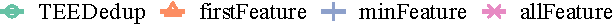
\includegraphics[width=0.7\linewidth]{pic/featurespy/plot/performance/multiClient/legend.pdf}\\
    \vspace{1pt}
    \begin{tabular}{@{\ }c@{\ }c@{\ }c}
            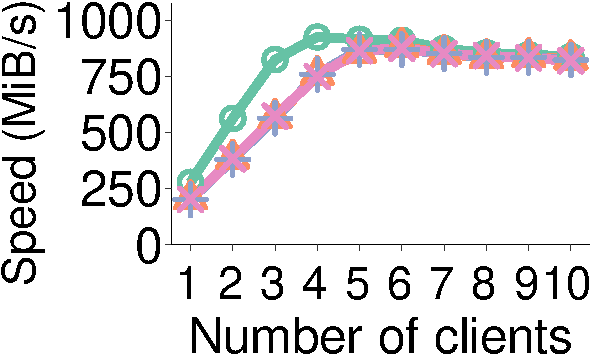
\includegraphics[width=0.32\textwidth]{pic/featurespy/plot/performance/multiClient/upload_1st_line.pdf}&
            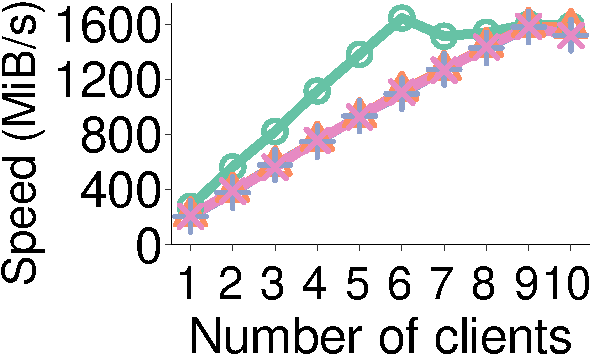
\includegraphics[width=0.32\textwidth]{pic/featurespy/plot/performance/multiClient/upload_2nd_line.pdf}&
            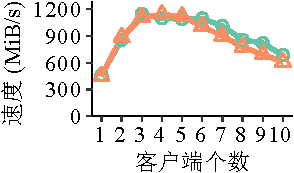
\includegraphics[width=0.32\textwidth]{pic/featurespy/plot/performance/multiClient/download_line.pdf}\\
            \makecell[c]{\small (a) 1st upload} &
            \makecell[c]{\small (b) 2nd upload} &
            \makecell[c]{\small (c) Download}\\
        \end{tabular}
        \vspace{-11pt}
        \captionof{figure}{(Exp\#8) 多客户端性能。 所有 \prototype 实例的下载速度都是相同的,我们将它(橙色)与 SGXDedup(绿色)进行比较。}
        \vspace{-5pt}
        \label{fig:expMultiClientThroughput}
\end{figure}

\begin{table}[t]
               \centering
                 \small
          \begin{tabular}{|c|c|c|c|}
                \hline
                {\bf Approach} & {\bf 1st Upload} & {\bf 2nd Upload} & {\bf Download} \\
                \hline
                \hline
                Transfer & \multicolumn{3}{c|}{11.8 $\pm$ 0.04} \\
                \hline
                \hline
                \makecell[c]{\tt firstFeature} & \multirow{3}{*}{11.5 $\pm$ 0.006} & 204.4 $\pm$ 10.06 & \multirow{3}{*}{11.5 $\pm$ 0.004} \\
                \cline{1-1}\cline{3-3}
                \makecell[c]{\tt minFeature} &  & 184.7$\pm$ 7.4 &  \\
                \cline{1-1}\cline{3-3}
                \makecell[c]{\tt allFeature} &  & 185.0$\pm$ 6.4 &  \\
                \hline
                SGXDedup & 11.5 $\pm$ 0.009 & 233.2 $\pm$ 8.4 & 11.5 $\pm$ 0.004 \\
                \hline
            \end{tabular}
        \vspace{2pt}
        \captionof{table}{(Exp\#7) 实云部署(单位:MiB/s)。 我们使用 {\tt scp} 将 2\,GiB 文件从客户端上传到云端,以提供环境中的传输基准。}
        \label{tab:expCloudTest}
\end{table}

图~\ref{fig:expMultiClientThroughput} 最多显示 10 个客户端的结果。我们不考虑更多的客户端,因为总体上传速度已经基本稳定。具体来说,第一次和第二次上传的速度都随着客户端数量的增加而增加,然后由于云端的写入竞争而逐渐降低。我们观察到 SGXDedup 比 \prototype 更早达到峰值性能(例如,四个客户端在第一次上传时达到 924.9\,MiB/s)(例如,在第一次上传中,六个客户端达到 882.2\,MiB/s),因为它实现了高性能并且云很容易饱和。类似地,由于读取云中的争用。


\paragraph{Exp\#8(实云部署)。}
我们扩展 Exp\#6 来研究云测试平台中的单客户端性能。我们将客户端和密钥服务器部署在同一地域的两台虚拟机中,以及不同地域的云中(相对于Exp\#7,所有实体都部署在同一地域),从而模拟场景Internet 连接在客户端和云之间。此外,我们让客户端从本地磁盘(即,读写速度约为 270\,MiB/s 用于读取/写入的 SSD)读取文件进行上传,云存储接收到的数据在附加的 NAS 中。我们使用 {\tt scp} 来对客户端和云之间的传输速度进行基准测试。


表~\ref{tab:expCloudTest} 显示了结果。在第一次上传中,所有方法的性能都受到传输速度的限制。在第二次上传中,SGXDedup 和 {\tt firstFeature} 的性能受到分块(Table~\ref{tab:evaluation-syn-system-breakdown})的限制,而 {\tt firstFeature} 产生 12.3\% 的性能开销SGXDedup,因为它额外提取了第一个特征来生成密钥。 {\tt minFeature} 和 {\tt allFeature}(在第二次上传中)的性能受特征提取的限制。请注意,所有方法的第二次上传速度都比 LAN 测试平台中的(Exp\#6)慢,原因有三个。首先,我们现在处理磁盘文件并启用磁盘 I/O。此外,云测试平台中的虚拟机是从物理机虚拟化的,在处理计算密集型操作时可能会导致性能下降。
此外,互联网的高延迟减慢了重复数据删除中指纹的传输速度。
在下载中,所有方法的性能都受到传输速度的限制,与 SGXDedup 相比,\prototype 会产生 0.6\% 的开销。


\subsubsection{实际工作负载}
\label{subsec:real}
我们使用 FSL 和 MS 评估 \prototype,以了解其在处理真实世界大规模数据时的性能。

\paragraph{Exp\#9(跟踪驱动的性能)。}
我们评估了 LAN 测试平台中的上传和下载性能。我们从 FSL 和 MS 中分别选择了 10 个快照,如下所示。对于 FSL,我们选择来自同一用户的每周快照以具有高交叉快照冗余;对于 MS,我们选择具有最多快照内冗余的快照。选择的 FSL 和 MS 快照分别采用 407.5\,GiB 和 902.5\,GiB 的预重复数据删除数据。由于我们的快照只包含块指纹和大小(\S\ref{sub:datasets}),我们通过重复将其指纹写入具有相应指定大小的备用块来重建每个明文块。我们先一张一张上传快照,然后按照上传的顺序下载。注意原来的 SGXDedup \cite{ren21} 没有容器缓存(\S\ref{sec:implementation});为了公平比较,我们为 SGXDedup 实现了一个内存缓存来缓冲最近恢复的容器,并将其配置为与 \prototype 相同的大小 (1\,GiB)。


\begin{figure}[t]
    \centering
    
\includegraphics[height=0.2in]{pic/featurespy/plot/performance/LANTrace/trace_legend_upload.pdf}\\
    
\includegraphics[height=0.2in]{pic/featurespy/plot/performance/LANTrace/trace_legend_download.pdf}\\
    \vspace{3pt}
    \begin{tabular}{@{\ }c@{\ }c}
        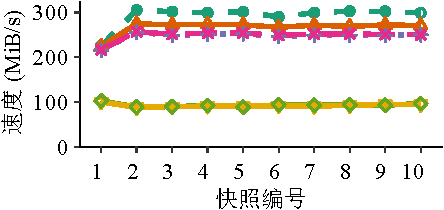
\includegraphics[width=0.47\textwidth]{pic/featurespy/plot/performance/LANTrace/trace_fsl.pdf}&
        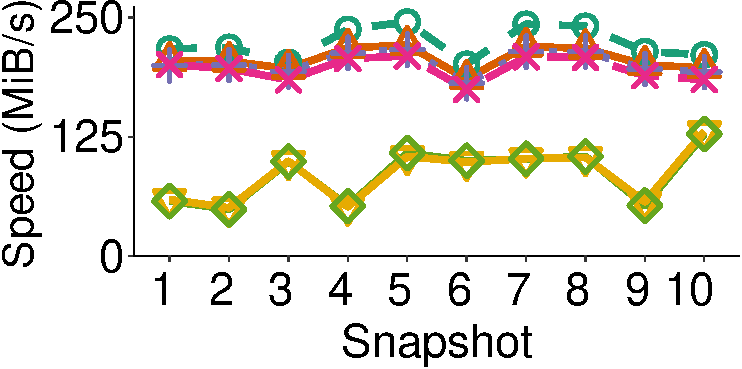
\includegraphics[width=0.47\textwidth]{pic/featurespy/plot/performance/LANTrace/trace_ms.pdf}\\
        \mbox{\small (a) FSL} &
        \mbox{\small (b) MS}\\
        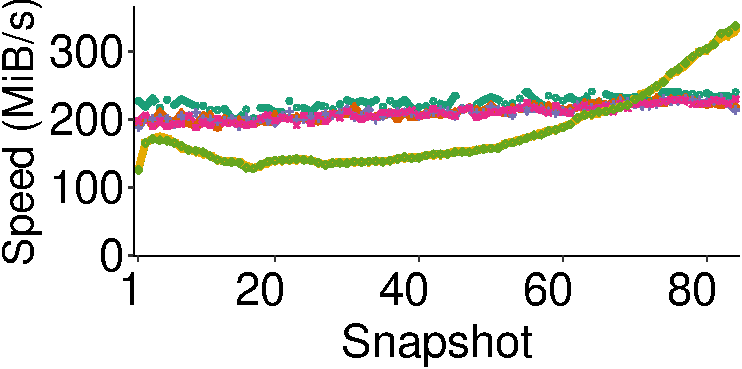
\includegraphics[width=0.47\textwidth]{pic/featurespy/plot/performance/LANTrace/trace_linux.pdf}&
        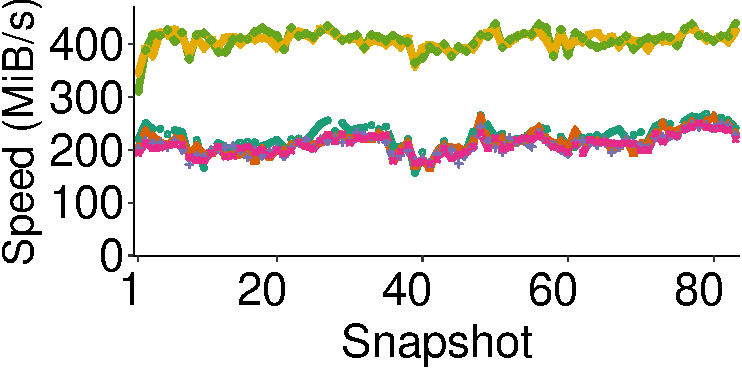
\includegraphics[width=0.47\textwidth]{pic/featurespy/plot/performance/LANTrace/trace_couch.pdf}\\
        \mbox{\small (c) Linux} &
        \mbox{\small (d) CouchDB}\\
    \end{tabular}
    \vspace{-6pt}
    \caption{(Exp\#9) Trace-driven performance.}
    \vspace{-6pt}
    \label{fig:traceDrivenThroughput}
\end{figure}
图~\ref{fig:traceDrivenThroughput} 展示了结果。在第一个 FSL 快照之后(例如,224.8\,MiB/s, 223.9\,MiB/s, 214.9\,MiB/s 和 216.9\,MiB/s 用于 SGXDedup、{\tt firstFeature}、{\tt minFeature} 和{\tt allFeature}),SGXDedup 和 \prototype 都实现了高性能(例如,至少 298.9\,MiB/s, 266.8\,MiB/s, 246.4\,MiB/s 和 248.8\,MiB/s SGXDedup、{\tt firstFeature}、{\tt minFeature} 和 {\tt allFeature}),因为它们不需要传输在 FSL 中占很大比例的交叉快照冗余。下载速度通常是稳定的(例如 SGXDedup 为 88.7-102.6\,MiB/s,\prototype 为 88.0-100.2\,MiB/s)。平均而言,与 SGXDedup 相比,{\tt firstFeature}、{\tt minFeature} 和 {\tt allFeature} 分别降低了上传性能 8.8\%、15.7\% 和 15.0\%,下载性能降低了 0.8 \%。

与 FSL 相比,MS 中的上传性能通常下降约 21\%,因为 MS 包含许多独特的块并导致较大的指纹索引(通过 LevelDB \cite{leveldb} 实现)。这加重了查询指纹索引是否存在密文块以进行重复数据删除的开销。此外,MS 中的下载速度会随着快照的变化而波动,因为一些快照具有更多的非重复块,并且可能存储在可以通过顺序读取快速访问的连续区域(即碎片较少的 \cite{lillibridge13})中。


\paragraph{Exp\#10(网络流量分析)。}
我们分析了 \prototype 的网络流量,并将其与三种可以抵御学习内容攻击的重复数据删除方法进行比较:(i) {\em target-based deduplication} \cite{harnik10},强制客户端传输所有密文块到云端; (ii) {\em random-threshold deduplication} \cite{harnik10},如果每个块的上传次数小于预定义的阈值,则执行基于存储目标的重复数据删除,或基于数据源的重复数据删除 (\S\ref {sub:basics}) 否则; (iii) {\em 两阶段重复数据删除} \cite{li15},它对来自同一客户端的密文块执行基于数据源的重复数据删除,然后对跨不同客户端的密文块执行基于存储目标的重复数据删除。在这里,我们按照之前的工作 \cite{harnik10} 分别在 20 和 2 处选择随机阈值重复数据删除中阈值的上限和下限。我们专注于 FSL 和 MS。对于 FSL,我们每天合并每个用户的快照,并按时间顺序存储。对于 MS,我们认为每个快照都来自一个单独的客户端,并按照快照 ID 的顺序存储快照。我们不考虑文件配方导致的带宽开销。

\begin{figure}[t]
    \centering
    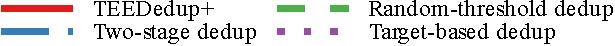
\includegraphics[width=0.8\textwidth]{pic/featurespy/plot/bandwidth/upload_traffic_legend.pdf}     \vspace{3pt} \\
    \begin{tabular}{@{\ }c@{\ }c}
        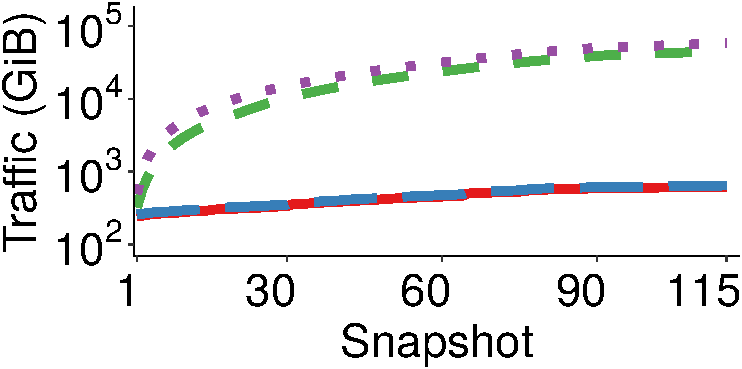
\includegraphics[width=0.47\textwidth]{pic/featurespy/plot/bandwidth/upload_traffic_fsl.pdf} &
        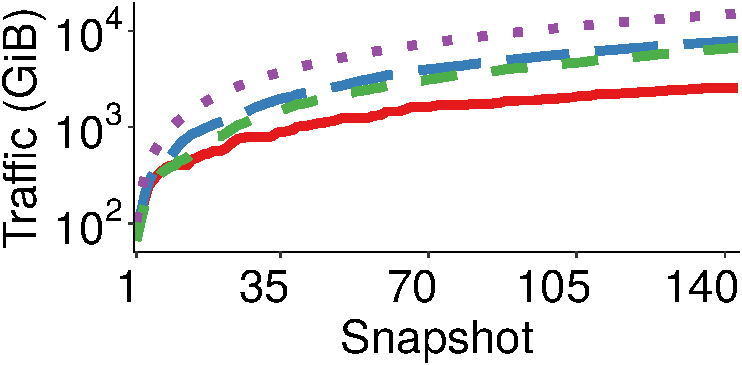
\includegraphics[width=0.47\textwidth]{pic/featurespy/plot/bandwidth/upload_traffic_ms.pdf} \\
        {\small (a) FSL} & {\small (b) MS} \\
        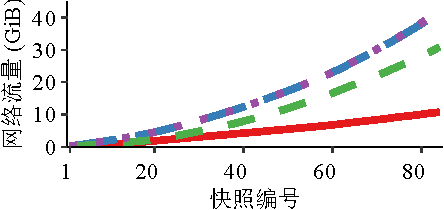
\includegraphics[width=0.47\textwidth]{pic/featurespy/plot/bandwidth/upload_traffic_linux.pdf} &
        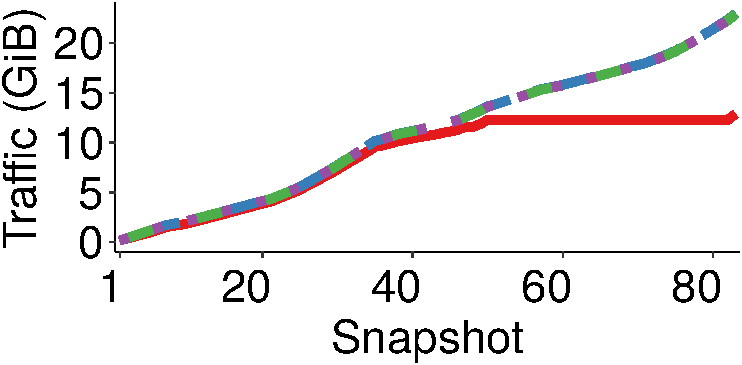
\includegraphics[width=0.47\textwidth]{pic/featurespy/plot/bandwidth/upload_traffic_couch.pdf} \\
        {\small (c) Linux} & {\small (d) CouchDB}
    \end{tabular}
    \vspace{-6pt}
    \caption{(Exp\#10) 存储每个快照后的累积网络流量。}
    \vspace{-6pt}
    \label{fig:expNetworkTraffic}
\end{figure}

图~\ref{fig:expNetworkTraffic} 展示了结果。由于 \prototype 执行纯基于数据源的重复数据删除,因此它优于其他方法。例如,在存储最后一个快照后,\prototype 将基于存储目标的重复数据删除的网络流量在 FSL 中减少了 98.9\%,在 MS 中减少了 83.1\%。两阶段重复数据删除在 ​​FSL 中表现良好(例如,只有 3.7\% 的带宽开销超过 \prototype),因为 FSL 包含大量用户内冗余。但是,在 MS 中,两级重复数据删除的网络流量最终是 \prototype 的 3.1$\times$。随机阈值重复数据删除会在 FSL(例如,\prototype 的 72.5$\times$)和 MS(例如,\prototype 的 2.6$\times$)中产生不同的网络流量。

由于 Linux 和 CouchDB 数据集的每个版本几乎没有冗余,并且需要大量基于数据源的重复数据删除查询,对于 Linux,它仅带来 $1.05\%$ 的流量节省,而对于 CouchDB,它甚至导致 $0.31 \%$ 额外的流量开销。随机阈值重复数据删除带来的流量节省是完全不同的。在 MS 中,它带来了 $55.75\%$ 的流量节省,而在 FSL 和 Linux 中,只有 $21.60\%$ 和 $26.68\%$。然而,它甚至在 CouchDB 中引入了 $0.0016\%$ 的额外流量开销。另外,我们发现在CouchDB的前35个版本中,几个方案的网络流量几乎是一样的,而对于后面的版本,\prototype 的累计网络流量几乎保持在一个水平。这是因为这 35 个版本是通用版本,几乎没有冗余。并且这些通用版本和社区/企业版本之间存在大量冗余,使得\prototype 不再需要上传大量数据。